% preamble start%
\documentclass[aspectratio=169,t,xcolor=table]{beamer}
\usepackage[utf8]{inputenc}

\usepackage{booktabs} 
\usepackage{subcaption}
\usepackage{blindtext}
\usepackage{hyperref}
\usetheme{Ufg}

%-------------------------------------theorems--------------
\newtheorem{conj}{Conjetura}
\newtheorem{defi}{Definição}
\newtheorem{teo}{Teorema}
\newtheorem{lema}{Lema}
\newtheorem{prop}{Proposição}
\newtheorem{cor}{Corolário}
\newtheorem{ex}{Exemplo}
\newtheorem{exer}{Exercício}

\setbeamertemplate{theorems}[numbered]
\setbeamertemplate{caption}[numbered]

%-------------------------------------------------------------%
%----------------------- Primary Definitions -----------------%

% This command set the default Color, is also possible to choose a custom color
\setPrimaryColor{LightGreen} 

% First one is logo in title slide (we recommend use a horizontal image), and second one is the logo used in the remaining slides (we recommend use a square image)
\setLogos{lib/logos/cast.png}{lib/logos/icrom.png} 


% -------------------------------------- Title Slide Information
%preamble end%
\begin{document}
\title[Inf UFG]{Bipedal Locomotion Optimization by Exploitation of the
Full Dynamics in DCM Trajectory Planning}
\subtitle{}

\author{Amirhosein Vedadi\inst{1}, Kasra Sinaei\inst{1, 2}, Pezhman Abdolahnezhad\inst{1}, \\
Shahriar Sheikh Aboumasoudi\inst{1}, Aghil Yousefi-Koma\inst{1}\\}
\institute[UFG] % (optional)
{
  \inst{1}%
  Center of Advanced Systems and Technologies (CAST)\\
  School of Mechanical Engineering\\
  University of Tehran\\
  \vspace{2mm}
  \inst{2}%
    Presentor
}
\date{November 2021}
%-----------------------The next statement creates the title page.
\frame[noframenumbering]{\titlepage}


%------------------------------------------------Slide 1
\setLayout{vertical} % This command define the layout. 'vertical' can be replace with 'horizontal', 'blank, 'mainpoint', 'titlepage'

\begin{frame}
    \frametitle{Table of Contents}
    \tableofcontents
\end{frame}
%---------------------------------------------------------
\section{Problem Statement}
%---------------------------------------------------------Slide 2
\setLayout{vertical}
\begin{frame}{Problem Statement}
    \begin{columns}
        \begin{column}{0.5\textwidth}
            Trajectory planning approaches:
            \begin{itemize}
                \item Full dynamic model
                \item Simplifed dynamic model\\
                {\begin{itemize}
                \item LIPM and DCM concepts
                \end{itemize}}
            \end{itemize}
            \vspace{3mm}
            In DCM trajectory planning, several parameters need to be set.\\
            \vspace{3mm}
            Simulation-based trajectory optimization considerations:
            \begin{itemize}
                \item Full dynamic model
                \item Foot-Ground contact model
            \end{itemize}

        \end{column}
        \begin{column}{0.6\textwidth}
            \begin{figure}
                \centering
                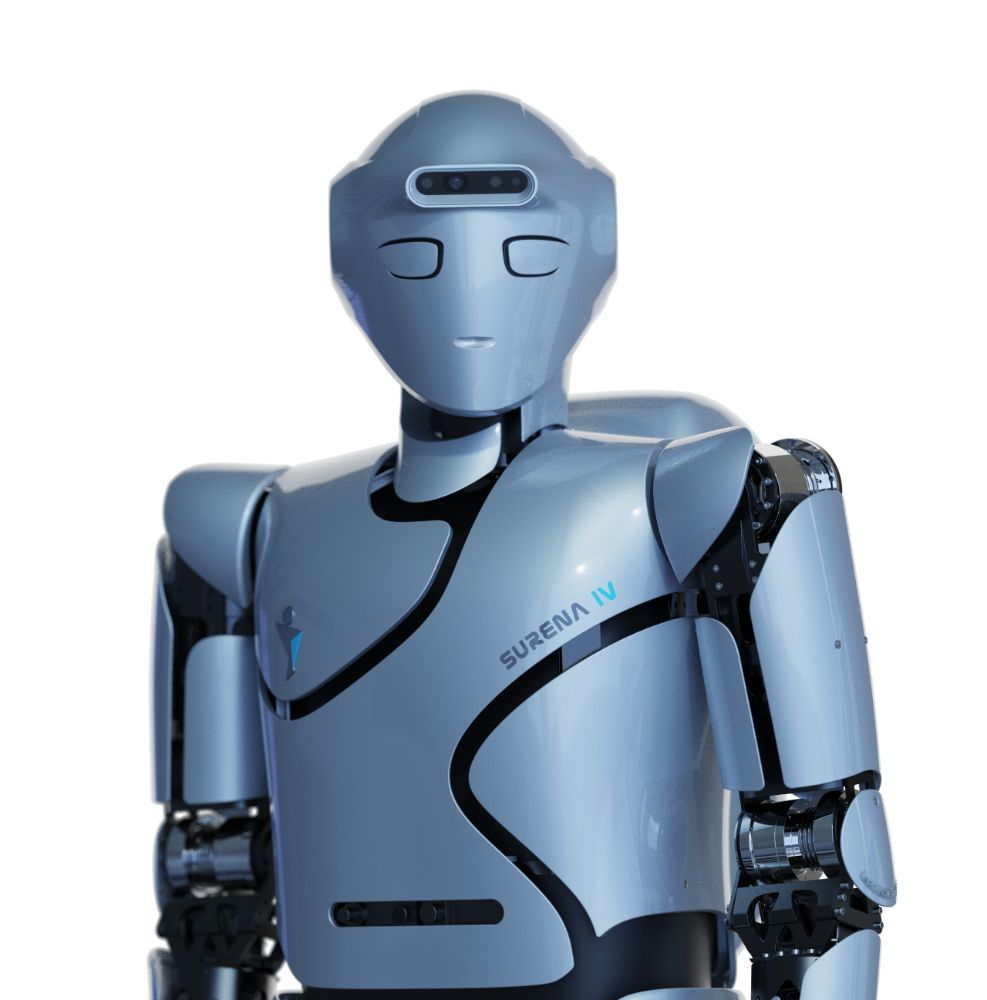
\includegraphics[height = 0.5\textheight]{lib/logos/SurenaIV.jpeg}
                \caption{Surena IV humanoid robot}
            \end{figure}
        \end{column}
    \end{columns}
\end{frame}

\section{DCM Based Trajectory Generation}

\setLayout{vertical}
\subsection{LIP Model and DCM Concept}
\begin{frame}{LIP Model and DCM Concept}
    LIPM Assumptions:
    \begin{itemize}
        \item Constant Height
        \item Concentrated Mass
        \item Zero Momentum about the Center of Mass
    \end{itemize}
    \begin{equation}
        \ddot{x} = \omega^{2}(x-r_{ZMP})
    \end{equation}
    Considering $\xi$ as a state variable:
    \begin{equation}
        \left\{
            \begin{matrix}
                \dot{\xi} = \omega(x-r_{ZMP})\\ 
                \dot{x} = -\omega(x-\xi)
            \end{matrix}
        \right.
    \end{equation}
    The first equation of (2) is unstable and that is why $\xi$ is called Divergent
    Component of Motion (DCM).
\end{frame}

\subsection{Trajectory Generation}
\begin{frame}{Trajectory Generation}
    DCM time domain equation:
    \begin{equation}
        \xi(t) = r_{ZMP} + e^{\sqrt{\frac{g}{z_0}}t}(\xi_{init} - r_{ZMP})
    \end{equation}
    Initial DCM positions are calculated recursively:
    \begin{equation}
        \xi_{init}^{i} = \xi_{end}^{i-1} = r_{ZMP}^i + e^{-\sqrt{\frac{g}{z_0}}t_{step}}(\xi_{end}^{i} - r_{ZMP}^i)
    \end{equation}
    for double support phase, we used a 3rd degree polynomial:
    \begin{equation}
        \left\{
            \begin{matrix}
                \xi_{init,DS}^{i} = r_{ZMP}^{i-1} + e^{-\sqrt{\frac{g}{z_0}}t_{(\Delta{t_{init,DS})}}}(\xi_{init}^{i} - r_{ZMP}^{i-1})\\ 
                \xi_{end,DS}^{i} = r_{ZMP}^{i} + e^{-\sqrt{\frac{g}{z_0}}t_{(\Delta{t_{end,DS})}}}(\xi_{init}^{i} - r_{ZMP}^{i})
            \end{matrix}
        \right.
    \end{equation}
    \begin{equation*}
        \Delta{t_{init,DS}}=\alpha t_{DS}, \Delta{t_{end,DS}}=(1-\alpha) t_{DS}
    \end{equation*}
\end{frame}

\begin{frame}{Trajectory Generation}
    CoM trajectory could be find by integrating the second equation of (2):
    \begin{equation}
        x(t)=e^{-\sqrt{\frac{g}{z_0}}t}(x(0)+\sqrt{\frac{g}{z_0}}\int{e^{\sqrt{\frac{g}{z_0}}t}}\xi(t)dt)    \end{equation}
    Also for ankle trajectories, we utilized a 5th degree polynomial.
    \begin{figure}
        \centering
        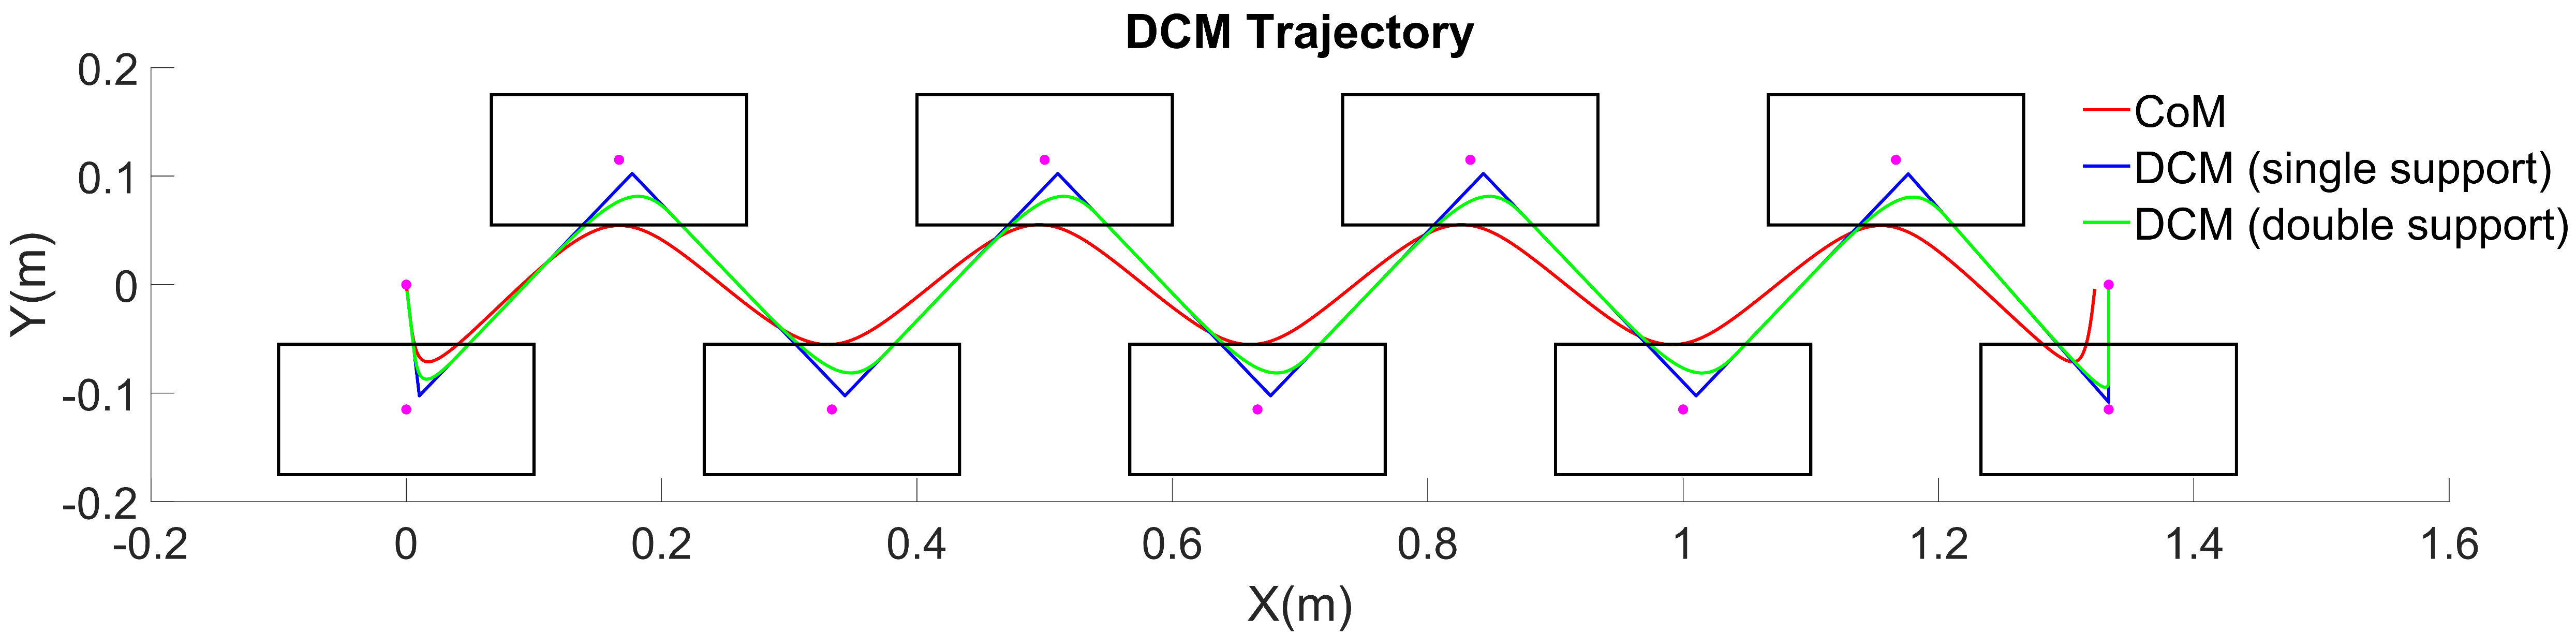
\includegraphics[width = 1.1\textheight]{lib/logos/DCMTrajectory.png}
        \caption{Schematic of planned trajectories}
    \end{figure}
\end{frame}

\section{Optimization Procedure}

\subsection{Optimization Problem}
\begin{frame}{Optimization Problem}
Optimization Parameters:
\begin{table}
\centering
\caption{Optimization Parameters and their search region}
\begin{tabular}{cccccc} 
\hline
    & $\alpha$ & $r_{DS}$ & $t_{step}(s)$ & $z_0(m)$ & $h_{ankle}(m)$  \\ 
\hline
min & 0.2      & 0.1      & 0.5           & 0.65     & 0.025           \\
max & 0.7      & 0.5      & 1.3           & 0.7      & 0.075           \\
\hline
\end{tabular}
\end{table}
Constraints:
	\begin{itemize}
        \item Robot's joints workspaces
        \item Maximum output torque of actuators
        \item Robot's center of mass height
        \item Constant walking speed
    \end{itemize}
\end{frame}

\begin{frame}{Optimization Problem}
Objective Functions:
\begin{equation}
J_E=-\sum_{i=1}^{12}E_i , J_{torque}=-\sum_{i=1}^{12}T_i , J_{vel}=-\sum_{i=1}^{12}\dot{q_i}  
\end{equation}
\begin{equation}
        \left\{
            \begin{matrix}
                J_{ZMP}=-r(p_{ZMP}, V)\ \ {if\ ZMP\ is\ inside}\\ 
                J_{ZMP}=r(p_{ZMP}, V)\ \ {if\ ZMP\ is\ not\ inside}
            \end{matrix}
        \right.
        \end{equation}
    \vspace{3mm}
    
These objective functions will be calculated during a
limited time (5s) of continuous walking on a straight
line by considering the full dynamics and foot-ground contact
models in PyBullet Simulation.
\end{frame}


\subsection{Single and Multi-Objective Optimization}
\begin{frame}{Single and Multi-Objective Optimization}
	\begin{itemize}
        \item First, each objective function optimized with the single objective GA
        \item With the help of multi-objective optimization, we can optimize $J_E$ and $J_{ZMP}$ simultaneously
    \end{itemize}
    \begin{table}
\centering
\caption{Optimization algorithms parameters}
\begin{tabular}{ccccc} 
\hline
Algorithm & \begin{tabular}[c]{@{}c@{}}Population \\size\end{tabular} & \begin{tabular}[c]{@{}c@{}}Crossover \\Type\end{tabular}         & \begin{tabular}[c]{@{}c@{}}Mutation \\Type\end{tabular} & Elitisms  \\ 
\hline
GA        & 100                                                       & Uniform (0.8)                                                    & Rand (0.08)                                             & 0.03      \\
NSGA-II   & 150                                                       & \begin{tabular}[c]{@{}c@{}}Simulated \\Binary (0.9)\end{tabular} & polynomial                                              & 0.0       \\
\hline
\end{tabular}
\end{table}
\end{frame}

\section{Results}

\subsection{ROS Based Framework}
\begin{frame}{ROS Based Framework}
    \begin{figure}
                \centering
                \includegraphics[height = 0.6\textheight]{lib/logos/framework.png}
                \caption{Schematic of the developed framework}
    \end{figure}
\end{frame}

\subsection{Single Objective Results}
\begin{frame}{Single Objective Results}
\begin{table}
\centering
\caption{Single objective optimization results}
\begin{tabular}{cccccc} 
\hline
$\alpha$ & $r_{DS}$ & $t_{step}$ & $z_0$ & $h_{ankle}$ & \begin{tabular}[c]{@{}c@{}}Objective\\Value\end{tabular}  \\ 
\hline
0.42     & 0.3      & 1.09          & 0.696    & 0.026          & $J_{E}=30.714 KJ$                                         \\
0.26     & 0.1      & 1.25          & 0.696    & 0.025          & $J_{torque}=3348 N.m$                                     \\
0.48     & 0.33     & 1.19          & 0.699    & 0.036          & $J_{vel}=155228\frac{rad}{s}$                             \\
0.38     & 0.1      & 0.6           & 0.658    & 0.036          & $J_{ZMP}=-132.54 m$                                       \\
\hline
\end{tabular}
\end{table}
\begin{itemize}
        \item $h_{ankle}$ and $z_0$ are almost equal to the minimum and maximum
values allowed for these parameters.
\item $J_E$ aligns with $J_{torque}$ and $J_{vel}$
    \end{itemize}
\end{frame}

\subsection{Multi-Objective Results}
\begin{frame}{Multi-Objective Results}
    \begin{figure}
        \centering
        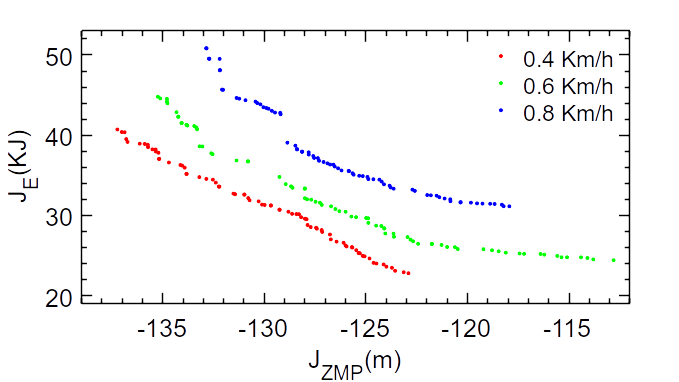
\includegraphics[width = 1\textheight]{lib/logos/ParetoSet.png}
        \caption{Pareto set of the multi-objective optimization}
    \end{figure}
\end{frame}

\begin{frame}{Multi-Objective Results}
The optimal parameters for some of the points which have
good results both in terms of energy and stability:
    \begin{table}
\centering
\caption{Multi-objective optimization results}
\begin{tabular}{ccccccc} 
\hline
\begin{tabular}[c]{@{}c@{}}speed\\($\frac{Km}{h}$)\end{tabular} & $\alpha$ & $r_{DS}$ & $t_{step}$ & $z_0$ & $h_{ankle}$ & \begin{tabular}[c]{@{}c@{}}Objective\\Values\end{tabular}  \\ 
\hline
0.4                                                             & 0.44     & 0.1      & 0.74       & 0.699 & 0.033       & $J_{E}=31.175 KJ,J_{ZMP}=-129.7m$                          \\
0.6                                                             & 0.69     & 0.1      & 1.05       & 0.677 & 0.025       & $J_{E}=32.079 KJ,J_{ZMP}=-127.9m$                          \\
0.8                                                             & 0.69     & 0.1      & 1.04       & 0.683 & 0.025       & $J_{E}=36.278 KJ,J_{ZMP}=-126.7m$                          \\
\hline
\end{tabular}
\end{table}
\end{frame}

\subsection{Choreonoid Simulation Results} 
\begin{frame}{Choreonoid Simulation Results}
    \begin{figure}
        \centering
        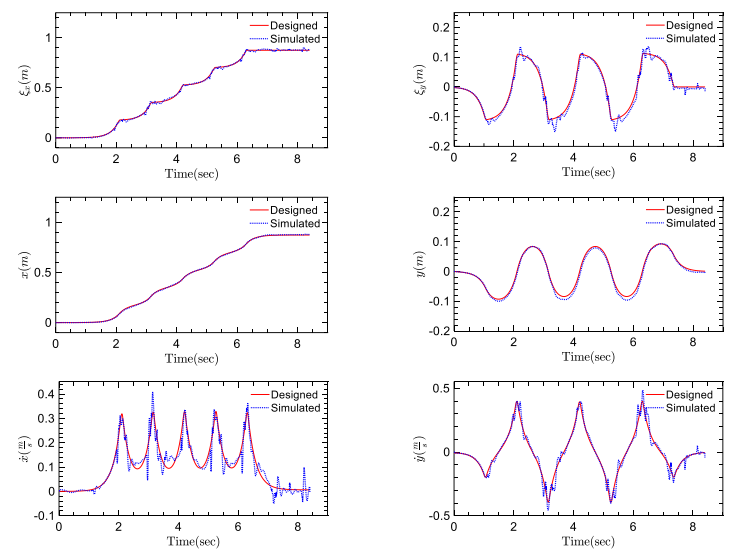
\includegraphics[width = 0.9\textheight]{lib/logos/choreonoid.png}
        \caption{Designed and simulated trajectories}
    \end{figure}
\end{frame}

\section{Conclusion}

\begin{frame}{Conclusion and Future Works}
    In this paperwe developed a framework to obtain optimal
parameters for trajectory planning based on DCM.
    \begin{itemize}
		\item We Considered full dynamic and foot-ground contact model in the simulation.
        \item With the help of the obtained results, we can design the robot trajectory to move online with the most stability or the lowest energy consumption.
		\item With the help of multi-objective optimization embedded in the
framework, we obtained trajectory parameters that compromise these two objectives at three different speeds.
\item We plan to design the optimal trajectory under different
conditions, such as moving on uneven and slippery surfaces
or soft surfaces for future works. And controlling robot’s motion while rejecting output
disturbances is another goal of the team for the future
    \end{itemize}
    
\end{frame}

\setLayout{blank}
\begin{frame}
    
    \centering
    \vspace{2cm}
    
    \textbf{\Huge Thanks}
    
    \ \\
    
    \textbf{Doubts and Suggestions}
    \ \\
    
    \text{\footnotesize https://github.com/CAST-Robotics/Trajectory-Optimization}
    \ \\
    
    \text{\footnotesize kasra.sinaei@ut.ac.ir}
    
    \vspace{0.5cm}
    \begin{figure}
        \centering
        
\includegraphics[height=1cm]{lib/logos/UofT.png}\\
        \vspace{0.5cm}
        
\includegraphics[height=1cm]{lib/logos/cast.png}\\
    \end{figure}
    
\end{frame}

%---------------------------------------------------------Slide 10
\setLayout{titlepage}
\setBGColor{DarkGray}
\titlepage
%-------------------------------------

\end{document}